%==========================================================
% CHAPTER 5: Stereometrija
%==========================================================
\chapter{Stereometrija (Erdvinė geometrija)}

\section{Tiesė ir plokštuma erdvėje}

Erdvinė geometrija nagrinėja tiesių ir plokštumų tarpusavio padėtis trimatėje erdvėje.
Analitiniam aprašymui naudojami \textbf{krypties vektoriai} ir \textbf{normalės vektoriai}.

\begin{definition}
Tiesės $T$ erdvėje \textbf{krypties vektorius} $\vec{s} = (l, m, n)$ yra bet kuris
vektorius, lygiagretus tai tiesei. Plokštumos $\alpha$ \textbf{normalės vektorius}
$\vec{n} = (A, B, C)$ yra vektorius, statmenas tai plokštumai.
\end{definition}

Tiesės erdvėje kanoninė lygtis, kai žinomas taškas $M_0(x_0, y_0, z_0)$ ir
krypties vektorius $\vec{s} = (l, m, n)$:
\[
  \frac{x - x_0}{l} = \frac{y - y_0}{m} = \frac{z - z_0}{n}.
\]
Plokštumos bendroji lygtis, kai žinomas normalės vektorius $\vec{n} = (A, B, C)$
ir taškas $M_0(x_0, y_0, z_0)$:
\[
  A(x - x_0) + B(y - y_0) + C(z - z_0) = 0,
\]
arba trumpiau:
\[
  Ax + By + Cz + D = 0.
\]

%------------------------------------------------------------------
\subsection{Lygiagretumo sąlygos}
%------------------------------------------------------------------

\subsubsection*{Dviejų tiesių lygiagrečiumas}

\begin{definition}
Dvi tiesės erdvėje vadinamos \textbf{lygiagrečiomis}, jei jos yra toje pačioje
plokštumoje ir nesusikerta.
\end{definition}

\begin{theorem}[Dviejų tiesių lygiagretumo sąlyga]
Tiesės $T_1$ ir $T_2$ su krypties vektoriais $\vec{s}_1 = (l_1, m_1, n_1)$ ir
$\vec{s}_2 = (l_2, m_2, n_2)$ yra \textbf{lygiagrečios} tada ir tik tada, kai
jų krypties vektoriai yra \emph{kolinearūs}, t.\,y.:
\[
  \frac{l_1}{l_2} = \frac{m_1}{m_2} = \frac{n_1}{n_2}.
\]
\end{theorem}

\begin{remark}
Kolinearumas reiškia, kad $\vec{s}_1 = k\,\vec{s}_2$ kažkokiam $k \in \mathbb{R}
\setminus \{0\}$. Taip pat reikia patikrinti, ar tiesės nesutampa (neturi
bendro taško).
\end{remark}

\begin{example}
Ar tiesės $T_1\colon \dfrac{x-1}{2} = \dfrac{y+3}{-4} = \dfrac{z}{6}$ ir
$T_2\colon \dfrac{x+2}{-1} = \dfrac{y}{2} = \dfrac{z-5}{-3}$ yra lygiagrečios?

\textit{Sprendimas.} Krypties vektoriai: $\vec{s}_1 = (2, -4, 6)$,
$\vec{s}_2 = (-1, 2, -3)$.
Patikriname:
\[
  \frac{2}{-1} = \frac{-4}{2} = \frac{6}{-3} = -2.
\]
Taip, visi santykiai lygūs $-2$, todėl $\vec{s}_1 = -2\,\vec{s}_2$.
Tiesės $T_1$ ir $T_2$ yra lygiagrečios (arba sutampančios -- tai reikia
papildomai patikrinti).
\end{example}

\subsubsection*{Tiesės ir plokštumos lygiagrečiumas}

\begin{theorem}[Tiesės ir plokštumos lygiagretumo sąlyga]
Tiesė $T$ su krypties vektoriumi $\vec{s} = (l, m, n)$ yra \textbf{lygiagreti}
plokštumai $\alpha\colon Ax + By + Cz + D = 0$ su normalės vektoriumi
$\vec{n} = (A, B, C)$ tada ir tik tada, kai $\vec{n} \perp \vec{s}$, t.\,y.:
\[
  \vec{n} \cdot \vec{s} = Al + Bm + Cn = 0.
\]
\end{theorem}

\begin{tcolorbox}[colback=blue!5!white, colframe=blue!40!black,
  title=Geometrinė prasmė]
Tiesė $T$ yra lygiagreti plokštumai $\alpha$, jei tiesė neturi jokio
bendro taško su plokštuma. Analitiškai tai reiškia, kad tiesės krypties
vektorius yra \emph{statmenas} plokštumos normalei.
\end{tcolorbox}

\begin{example}
Nustatyti, su kuria $B$ reikšme tiesė
$T\colon \dfrac{x-1}{3} = \dfrac{y+2}{B} = \dfrac{z}{-1}$
yra lygiagreti plokštumai $\alpha\colon 2x - y + 4z - 5 = 0$.

\textit{Sprendimas.} $\vec{s} = (3, B, -1)$, $\vec{n} = (2, -1, 4)$.
Taikome lygiagretumo sąlygą:
\[
  \vec{n} \cdot \vec{s} = 2 \cdot 3 + (-1) \cdot B + 4 \cdot (-1) = 0
  \implies 6 - B - 4 = 0 \implies B = 2.
\]
\end{example}

\subsubsection*{Dviejų plokštumų lygiagrečiumas}

\begin{theorem}[Dviejų plokštumų lygiagretumo sąlyga]
Plokštumos $\alpha_1\colon A_1 x + B_1 y + C_1 z + D_1 = 0$ ir
$\alpha_2\colon A_2 x + B_2 y + C_2 z + D_2 = 0$ yra \textbf{lygiagrečios}
tada ir tik tada, kai jų normalės vektoriai
$\vec{n}_1 = (A_1, B_1, C_1)$ ir $\vec{n}_2 = (A_2, B_2, C_2)$ yra
\emph{kolinearūs}:
\[
  \frac{A_1}{A_2} = \frac{B_1}{B_2} = \frac{C_1}{C_2}.
\]
Papildoma sąlyga: plokštumos nesutampa, t.\,y.
$\dfrac{A_1}{A_2} = \dfrac{B_1}{B_2} = \dfrac{C_1}{C_2} \neq \dfrac{D_1}{D_2}$.
\end{theorem}

\begin{remark}
Jei $\dfrac{A_1}{A_2} = \dfrac{B_1}{B_2} = \dfrac{C_1}{C_2} = \dfrac{D_1}{D_2}$,
tai plokštumos \emph{sutampa}.
\end{remark}

\begin{theorem}[Stereometrinė lygiagretumo teorema]
Tiesė yra lygiagreti plokštumai, jei ji yra lygiagreti bent vienai toje
plokštumoje gulinčiai tiesei.

Dvi plokštumos yra lygiagrečios, jei dvi susikertančios vienos plokštumos
tiesės yra lygiagrečios atitinkamoms kitos plokštumos tiesėms.
\end{theorem}

%------------------------------------------------------------------
\subsection{Statmenumo sąlygos}
%------------------------------------------------------------------

\subsubsection*{Dviejų tiesių statmenumo erdvėje sąlyga}

\begin{theorem}[Dviejų tiesių statmenumo sąlyga]
Tiesės $T_1$ ir $T_2$ su krypties vektoriais $\vec{s}_1 = (l_1, m_1, n_1)$ ir
$\vec{s}_2 = (l_2, m_2, n_2)$ yra \textbf{statmenos} tada ir tik tada, kai
$\vec{s}_1 \perp \vec{s}_2$, t.\,y. jų skaliarinė sandauga lygi nuliui:
\[
  \vec{s}_1 \cdot \vec{s}_2 = l_1 l_2 + m_1 m_2 + n_1 n_2 = 0.
\]
\end{theorem}

\begin{remark}
Erdvėje dvi tiesės gali būti \emph{susikertančios} ir statmenos arba
\emph{pasikertančios} (neturinčios bendro taško, bet krypties vektoriai
statmeni). Abiem atvejais statmenumo sąlyga ta pati.
\end{remark}

\begin{example}
Ar tiesės $T_1\colon \dfrac{x}{1} = \dfrac{y-1}{2} = \dfrac{z+2}{-3}$ ir
$T_2\colon \dfrac{x-4}{3} = \dfrac{y+1}{0} = \dfrac{z}{1}$ yra statmenos?

\textit{Sprendimas.} $\vec{s}_1 = (1, 2, -3)$, $\vec{s}_2 = (3, 0, 1)$.
\[
  \vec{s}_1 \cdot \vec{s}_2 = 1 \cdot 3 + 2 \cdot 0 + (-3) \cdot 1 = 3 + 0 - 3 = 0.
\]
Skaliarinė sandauga lygi nuliui, taigi tiesės yra statmenos.
\end{example}

\subsubsection*{Tiesės ir plokštumos statmenumo sąlyga}

\begin{theorem}[Tiesės ir plokštumos statmenumo sąlyga]
Tiesė $T$ su krypties vektoriumi $\vec{s} = (l, m, n)$ yra \textbf{statmena}
plokštumai $\alpha\colon Ax + By + Cz + D = 0$ su normalės vektoriumi
$\vec{n} = (A, B, C)$ tada ir tik tada, kai $\vec{s}$ ir $\vec{n}$ yra
\emph{kolinearūs}, t.\,y. jų koordinatės proporcingos:
\[
  \frac{A}{l} = \frac{B}{m} = \frac{C}{n}.
\]
\end{theorem}

\begin{tcolorbox}[colback=green!5!white, colframe=green!40!black,
  title=Geometrinė prasmė]
Tiesė $T$ yra statmena plokštumai $\alpha$, jei $T$ yra statmena
\emph{kiekvienai} plokštumos tiesei. Analitiškai tai reiškia, kad tiesės
krypties vektorius yra \emph{lygiagretus} plokštumos normalei.
\end{tcolorbox}

\begin{example}
Sudaryti plokštumos, einančios per tašką $M_0(1, -2, 3)$ ir statmenos
tiesei $T\colon \dfrac{x-5}{2} = \dfrac{y}{-1} = \dfrac{z+1}{4}$, lygtį.

\textit{Sprendimas.} Kadangi plokštuma statmena tiesei $T$, tai plokštumos
normalė $\vec{n}$ lygiagreti tiesės krypties vektoriui:
$\vec{n} = \vec{s} = (2, -1, 4)$.

Plokštumos lygtis per tašką $M_0(1, -2, 3)$:
\[
  2(x - 1) + (-1)(y + 2) + 4(z - 3) = 0
  \implies 2x - y + 4z - 16 = 0.
\]
\end{example}

\subsubsection*{Dviejų plokštumų statmenumo sąlyga}

\begin{theorem}[Dviejų plokštumų statmenumo sąlyga]
Plokštumos $\alpha_1$ ir $\alpha_2$ su normalės vektoriais
$\vec{n}_1 = (A_1, B_1, C_1)$ ir $\vec{n}_2 = (A_2, B_2, C_2)$
yra \textbf{statmenos} tada ir tik tada, kai $\vec{n}_1 \perp \vec{n}_2$:
\[
  \vec{n}_1 \cdot \vec{n}_2 = A_1 A_2 + B_1 B_2 + C_1 C_2 = 0.
\]
\end{theorem}

\begin{theorem}[Dviejų plokštumų statmenumo teorema -- stereometrinė]
Jei viena iš dviejų plokštumų eina per tiesę, statmeną kitai plokštumai,
tai tos dvi plokštumos yra statmenos viena kitai. Simboliškai:
\[
  \text{jei } m \perp \alpha \text{ ir } m \in \beta,
  \text{ tai } \beta \perp \alpha.
\]
\end{theorem}

\begin{theorem}[Trijų statmenų teorema]
Jei plokštumos tiesė $a$, einanti per pasvirosios $AC$ pagrindą $C$, yra
statmena pasvirosios projekcijai $BC$ plokštumoje $\alpha$, tai ji yra
statmena ir pačiai pasvirajai $AC$:
\[
  \text{jei } AB \perp \alpha,\; a \in \alpha,\; a \perp BC,
  \text{ tai } a \perp AC.
\]
čia $AC$ -- pasviroji, $BC$ -- pasvirosios projekcija, $a$ -- plokštumos tiesė.
\end{theorem}

\subsubsection*{Lygiagretumo ir statmenumo sąlygų suvestinė}

\begin{center}
\begin{tabular}{|l|c|c|}
\hline
\textbf{Objektai} & \textbf{Lygiagrečiumas} & \textbf{Statmenumo} \\
\hline
Dvi tiesės
  & $\dfrac{l_1}{l_2} = \dfrac{m_1}{m_2} = \dfrac{n_1}{n_2}$
  & $l_1 l_2 + m_1 m_2 + n_1 n_2 = 0$ \\[8pt]
\hline
Tiesė ir plokštuma
  & $Al + Bm + Cn = 0$
  & $\dfrac{A}{l} = \dfrac{B}{m} = \dfrac{C}{n}$ \\[8pt]
\hline
Dvi plokštumos
  & $\dfrac{A_1}{A_2} = \dfrac{B_1}{B_2} = \dfrac{C_1}{C_2}$
  & $A_1 A_2 + B_1 B_2 + C_1 C_2 = 0$ \\[8pt]
\hline
\end{tabular}
\end{center}

\begin{exercise}
Duota plokštuma $\alpha\colon 3x - 2y + z - 6 = 0$.
\begin{enumerate}[label=\alph*)]
  \item Suraskite plokštumai lygiagrečią plokštumą, einančią per tašką $P(1,0,-1)$.
  \item Parašykite tiesės, einančios per tašką $P(1,0,-1)$ ir statmenos plokštumai
        $\alpha$, kanoninę lygtį.
\end{enumerate}
\end{exercise}

\begin{exercise}
Įrodykite, kad tiesė $T\colon \dfrac{x-2}{1} = \dfrac{y-1}{-3} = \dfrac{z+4}{2}$
yra lygiagreti plokštumai $\alpha\colon x + y + z - 1 = 0$ ir raskite
atstumą nuo tiesės iki plokštumos.
\end{exercise}

\begin{exercise}
Tiesė $T$ eina per taškus $A(1, 2, -1)$ ir $B(3, 0, 2)$.
Plokštuma $\alpha$ eina per taškus $P(0,0,0)$, $Q(1,1,0)$, $R(0,1,1)$.
Nustatykite tiesės ir plokštumos tarpusavio padėtį.
\end{exercise}


\section{Daugiasieniai}

\begin{definition}
\textbf{Daugiasieniai} (arba \textbf{briaunainiai}) --- erdvinės figūros, kurių visi paviršiai yra daugiakampiai. Kiekvienas toks daugiakampis vadinamas \textit{sienele}, gretimų sienelių bendroji atkarpa --- \textit{briauna}, o gretimų briaunų bendras taškas --- \textit{viršūne}.
\end{definition}

% ─────────────────────────────────────────
\subsection{Prizmės}
% ─────────────────────────────────────────

\begin{definition}
\textbf{Prizmė} --- daugiasienio, kurio dvi sienelės (vadinamos \textit{pagrindais}) yra lygūs ir lygiagrečiai išdėstyti daugiakampiai, o likusios sienelės (vadinamos \textit{šoninėmis sienomis}) yra lygiagretainiai.
\end{definition}

\begin{definition}
\textbf{Prizmės aukštine} vadinama statmuo, nubrėžtas iš vieno pagrindo plokštumos į kitą. Aukštinės ilgis žymimas $H$.
\end{definition}

\subsubsection*{Prizmių rūšys}

\begin{itemize}
    \item \textbf{Stačioji prizmė} --- prizmė, kurios šoninės briaunos statmenos pagrindams, t.~y.\ $AA_1 \perp$ pagrindo plokštumai. Tokiu atveju šoninės sienos yra stačiakampiai, o šoninės briaunos ilgis lygus aukštinei: $|AA_1| = H$.
    \item \textbf{Pasviroji prizmė} --- prizmė, kurios šoninės briaunos nėra statmenos pagrindams.
    \item \textbf{Taisyklingoji prizmė} --- stačioji prizmė, kurios pagrindai yra taisyklingieji daugiakampiai.
    \item \textbf{Gretasienis} --- keturkampė prizmė (abu pagrindai yra lygiagretainiai).
    \item \textbf{Stačiakampis gretasienis} --- stačioji prizmė, kurios pagrindai yra stačiakampiai.
    \item \textbf{Kubas} --- stačiakampis gretasienis, kurio visos briaunos lygios.
\end{itemize}

\subsubsection*{Prizmės paviršiaus plotas}

\begin{definition}
\textbf{Prizmės paviršiaus plotu} vadinama visų jos sienelių plotų suma. \textbf{Šoninio paviršiaus plotu} --- tik šoninių sienų plotų suma.
\end{definition}

Stačiosios prizmės šoninės sienos yra stačiakampiai, todėl kiekvienos šoninės sienos plotas lygus $a_i \cdot H$, kur $a_i$ --- atitinkama pagrindo kraštinė. Sudėję visų šoninių sienų plotus gauname:

\begin{tcolorbox}[colback=blue!5!white, colframe=blue!50!black, title=Stačiosios prizmės šoninis paviršiaus plotas]
\[
    S_{\text{šon}} = P \cdot H,
\]
kur $P$ --- pagrindo perimetras, $H$ --- aukštinė.
\end{tcolorbox}

\begin{tcolorbox}[colback=blue!5!white, colframe=blue!50!black, title=Viso paviršiaus plotas]
\[
    S = S_{\text{šon}} + 2S_{\text{pagr}},
\]
kur $S_{\text{pagr}}$ --- vieno pagrindo plotas.
\end{tcolorbox}

\begin{remark}
Pasvirosios prizmės atveju šoninių sienų plotui apskaičiuoti naudojamas \textbf{statmenasis pjūvis} --- pjūvis, statmenas visoms šoninėms briaunoms. Jei $Q$ --- statmenojo pjūvio plotas, o $l$ --- šoninės briaunos ilgis, tai:
\[
    S_{\text{šon}} = P_{\perp} \cdot l,
\]
kur $P_{\perp}$ --- statmenojo pjūvio perimetras.
\end{remark}

\subsubsection*{Prizmės tūris}

\begin{tcolorbox}[colback=green!5!white, colframe=green!50!black, title=Prizmės tūrio formulė]
\[
    V = S_{\text{pagr}} \cdot H,
\]
kur $S_{\text{pagr}}$ --- pagrindo plotas, $H$ --- aukštinė.
\end{tcolorbox}

\begin{remark}
Pasvirosios prizmės tūris gali būti išreikštas per statmenąjį pjūvį:
\[
    V = Q \cdot l,
\]
kur $Q$ --- statmenojo pjūvio plotas, $l$ --- šoninės briaunos ilgis.
\end{remark}

\subsubsection*{Ypatingos prizmių formulės}

\begin{center}
\renewcommand{\arraystretch}{1.8}
\begin{tabular}{|l|c|c|}
\hline
\textbf{Figūra} & \textbf{Paviršiaus plotas $S$} & \textbf{Tūris $V$} \\
\hline
Kubas (briauna $a$) & $6a^2$ & $a^3$ \\
\hline
Stačiakampis gretasienis ($a, b, c$) & $2(ab + bc + ac)$ & $abc$ \\
\hline
Taisyklingoji trikampė prizmė (briauna $a$, aukštinė $H$) & $3aH + \dfrac{\sqrt{3}}{2}a^2$ & $\dfrac{\sqrt{3}}{4}a^2 H$ \\
\hline
Taisyklingoji šešiakampė prizmė (briauna $a$, aukštinė $H$) & $6aH + 3\sqrt{3}a^2$ & $\dfrac{3\sqrt{3}}{2}a^2 H$ \\
\hline
\end{tabular}
\end{center}

\subsubsection*{Uždavinių pavyzdžiai}

\begin{example}
Taisyklingosios trikampės prizmės pagrindo kraštinė $a = 6$ cm, o aukštinė $H = 10$ cm. Raskite prizmės tūrį ir viso paviršiaus plotą.

\textbf{Sprendimas.}

Pagrindo plotas (lygiakraščio trikampio):
\[
    S_{\text{pagr}} = \frac{\sqrt{3}}{4} a^2 = \frac{\sqrt{3}}{4} \cdot 36 = 9\sqrt{3} \text{ cm}^2.
\]

Tūris:
\[
    V = S_{\text{pagr}} \cdot H = 9\sqrt{3} \cdot 10 = 90\sqrt{3} \approx 155{,}88 \text{ cm}^3.
\]

Pagrindo perimetras: $P = 3 \cdot 6 = 18$ cm.

Šoninis paviršiaus plotas:
\[
    S_{\text{šon}} = P \cdot H = 18 \cdot 10 = 180 \text{ cm}^2.
\]

Visas paviršiaus plotas:
\[
    S = S_{\text{šon}} + 2S_{\text{pagr}} = 180 + 2 \cdot 9\sqrt{3} = 180 + 18\sqrt{3} \approx 211{,}18 \text{ cm}^2.
\]
\end{example}

\begin{example}
Stačiakampio gretasienio matmenys: $a = 3$ cm, $b = 4$ cm, $c = 5$ cm. Raskite įstrižainės ilgį.

\textbf{Sprendimas.}

Stačiakampio gretasienio įstrižainė:
\[
    d = \sqrt{a^2 + b^2 + c^2} = \sqrt{9 + 16 + 25} = \sqrt{50} = 5\sqrt{2} \approx 7{,}07 \text{ cm}.
\]
\end{example}

\begin{exercise}
Stačiosios prizmės pagrindas yra stačiakampis, kurio kraštinės $3$ cm ir $4$ cm. Prizmės įstrižainė sudaro $45°$ kampą su pagrindu. Raskite prizmės tūrį.
\end{exercise}

% ─────────────────────────────────────────
\subsection{Piramidės}
% ─────────────────────────────────────────

\begin{definition}
\textbf{Piramidė} --- daugiasienio, kurio viena sienelė (vadinama \textit{pagrindu}) yra daugiakampis, o visos kitos sienelės (vadinamos \textit{šoninėmis sienomis}) yra trikampiai, turintys bendrą viršūnę $S$, vadinama \textit{piramidės viršūne}.
\end{definition}

\begin{definition}
\textbf{Piramidės aukštine} vadinama atkarpa $SH$, kur $H$ yra viršūnės $S$ projekcija į pagrindo plokštumą ($SH \perp$ pagrindo plokštumai). Aukštinės ilgis žymimas $h$ arba $H$.
\end{definition}

\subsubsection*{Piramidžių rūšys}

\begin{itemize}
    \item \textbf{Taisyklingoji piramidė} --- piramidė, kurios pagrindas yra taisyklingasis daugiakampis, o aukštinė eina per pagrindo centrą (sutampa su pagrindo simetrijos ašimi).
    \item \textbf{Trikampė piramidė (tetraedras)} --- piramidė, kurios pagrindas yra trikampis; visos keturios sienelės yra trikampiai.
    \item \textbf{Taisyklingasis tetraedras} --- tetraedras, kurio visos keturios sienelės yra vienodi lygiakraščiai trikampiai.
    \item \textbf{Nupjautinė piramidė} --- figūra, gaunama nupjovus piramidę plokštuma, lygiagrečia pagrindui.
\end{itemize}

\subsubsection*{Svarbūs elementai}

\begin{definition}
Taisyklingosios piramidės \textbf{apotema} $h_a$ --- tai šoninės sienelės (trikampio) aukštinė, nuleista iš viršūnės į pagrindo kraštinę. Tai kartu yra ir trumpiausias atstumas nuo viršūnės iki pagrindo kraštinės.
\end{definition}

Taisyklingosios $n$-kampės piramidės apotemai taikoma Pitagoro teorema:
\[
    h_a^2 = H^2 + r^2,
\]
kur $H$ --- aukštinės ilgis, $r$ --- pagrindu įbrėžto apskritimo spindulys.

Analogiškai šoninės briaunos ilgiui:
\[
    l^2 = H^2 + R^2,
\]
kur $R$ --- pagrindu apibrėžto apskritimo spindulys.

\subsubsection*{Piramidės tūris}

\begin{tcolorbox}[colback=green!5!white, colframe=green!50!black, title=Piramidės tūrio formulė]
\[
    V = \frac{1}{3} S_{\text{pagr}} \cdot H,
\]
kur $S_{\text{pagr}}$ --- pagrindo plotas, $H$ --- aukštinė.
\end{tcolorbox}

\begin{remark}
Piramidės tūris lygus vienai trečdaliai prizmės, turėjusios tokį pat pagrindą ir aukštinę, tūrio. Tai yra fundamentalus geometrijos rezultatas.
\end{remark}

\subsubsection*{Piramidės paviršiaus plotas}

\begin{tcolorbox}[colback=blue!5!white, colframe=blue!50!black, title=Taisyklingosios piramidės šoninis paviršiaus plotas]
\[
    S_{\text{šon}} = \frac{1}{2} P \cdot h_a,
\]
kur $P$ --- pagrindo perimetras, $h_a$ --- apotema (šoninės sienelės aukštinė).
\end{tcolorbox}

\begin{tcolorbox}[colback=blue!5!white, colframe=blue!50!black, title=Viso paviršiaus plotas]
\[
    S = S_{\text{šon}} + S_{\text{pagr}}.
\]
\end{tcolorbox}

\subsubsection*{Taisyklingasis tetraedras}

Taisyklingojo tetraedro (visos briaunos lygios $a$) formulės:

\begin{center}
\renewcommand{\arraystretch}{1.8}
\begin{tabular}{|l|c|}
\hline
\textbf{Dydis} & \textbf{Formulė} \\
\hline
Vienos sienelės plotas & $\dfrac{\sqrt{3}}{4}a^2$ \\
\hline
Viso paviršiaus plotas & $\sqrt{3}\, a^2$ \\
\hline
Aukštinė & $H = a\sqrt{\dfrac{2}{3}}$ \\
\hline
Tūris & $V = \dfrac{a^3\sqrt{2}}{12}$ \\
\hline
Apibrėžto apskritimo spindulys & $R = \dfrac{a\sqrt{6}}{4}$ \\
\hline
Įbrėžto apskritimo spindulys & $r = \dfrac{a\sqrt{6}}{12}$ \\
\hline
\end{tabular}
\end{center}

\subsubsection*{Nupjautinė piramidė}

\begin{definition}
\textbf{Nupjautinė piramidė} --- figūra tarp piramidės pagrindo ir plokštumos, lygiagrečios pagrindui ir kertančios visas šonines briaunas. Jos pagrindai yra du panašūs daugiakampiai su plotais $S_1$ (didelis) ir $S_2$ (mažas), o aukštinė --- $H$.
\end{definition}

\begin{tcolorbox}[colback=green!5!white, colframe=green!50!black, title=Nupjautinės piramidės tūris]
\[
    V = \frac{H}{3}\left(S_1 + \sqrt{S_1 S_2} + S_2\right),
\]
kur $S_1$, $S_2$ --- pagrindų plotai, $H$ --- aukštinė.
\end{tcolorbox}

\begin{tcolorbox}[colback=blue!5!white, colframe=blue!50!black, title=Taisyklingosios nupjautinės piramidės šoninis paviršiaus plotas]
\[
    S_{\text{šon}} = \frac{1}{2}(P_1 + P_2) \cdot h_a,
\]
kur $P_1$, $P_2$ --- pagrindų perimetrai, $h_a$ --- apotema (šoninės trapecijos aukštinė).
\end{tcolorbox}

\subsubsection*{Uždavinių pavyzdžiai}

\begin{example}
Taisyklingosios keturkampės piramidės pagrindo kraštinė $a = 6$ cm, o aukštinė $H = 4$ cm. Raskite tūrį ir viso paviršiaus plotą.

\textbf{Sprendimas.}

Pagrindo plotas (kvadratas):
\[
    S_{\text{pagr}} = a^2 = 36 \text{ cm}^2.
\]

Tūris:
\[
    V = \frac{1}{3} S_{\text{pagr}} \cdot H = \frac{1}{3} \cdot 36 \cdot 4 = 48 \text{ cm}^3.
\]

Apotemos ilgis (įbrėžto apskritimo spindulys $r = a/2 = 3$ cm):
\[
    h_a = \sqrt{H^2 + r^2} = \sqrt{16 + 9} = \sqrt{25} = 5 \text{ cm}.
\]

Šoninis paviršiaus plotas:
\[
    S_{\text{šon}} = \frac{1}{2} P \cdot h_a = \frac{1}{2} \cdot 24 \cdot 5 = 60 \text{ cm}^2.
\]

Visas paviršiaus plotas:
\[
    S = S_{\text{šon}} + S_{\text{pagr}} = 60 + 36 = 96 \text{ cm}^2.
\]
\end{example}

\begin{example}
Nupjautinės taisyklingosios keturkampės piramidės pagrindų kraštinės yra $a_1 = 8$ cm ir $a_2 = 4$ cm, aukštinė $H = 6$ cm. Raskite tūrį.

\textbf{Sprendimas.}

Pagrindų plotai:
\[
    S_1 = 8^2 = 64 \text{ cm}^2, \quad S_2 = 4^2 = 16 \text{ cm}^2.
\]

Tūris:
\[
    V = \frac{H}{3}(S_1 + \sqrt{S_1 S_2} + S_2) = \frac{6}{3}(64 + \sqrt{64 \cdot 16} + 16) = 2(64 + 32 + 16) = 2 \cdot 112 = 224 \text{ cm}^3.
\]
\end{example}

\begin{exercise}
Taisyklingosios trikampės piramidės visų briaunų ilgiai lygūs $a$. Raskite piramidės tūrį ir viso paviršiaus plotą, išreikštus per $a$.
\end{exercise}

\begin{exercise}
Piramidės pagrindas yra stačiakampis, kurio kraštinės $3$ cm ir $4$ cm. Viena iš šoninių briaunų statmena pagrindui ir lygi $6$ cm. Raskite piramidės tūrį.
\end{exercise}


\section{Sukimosi kūnai}

Sukimosi kūnai yra erdvinės figūros, gaunamos sukant plokštuminę figūrą aplink tiesią ašį, vadinamą \textbf{sukimosi ašimi}. Pagrindiniai sukimosi kūnai yra \textbf{cilindras}, \textbf{kūgis} ir \textbf{rutulys}.

% ──────────────────────────────────────────────
\subsection{Cilindras}
% ──────────────────────────────────────────────

\begin{definition}
\textbf{Stačiasis cilindras} – tai sukimosi kūnas, gaunamas sukant stačiakampį aplink vieną iš jo kraštinių. Cilindras turi du lygiagrečius, vienodus apskritus pagrindus ir šoninį paviršių.
\end{definition}

\subsubsection*{Pagrindiniai elementai}

\begin{itemize}
    \item $r$ – pagrindo apskritimo spindulys,
    \item $h$ – cilindro aukštis (atstumas tarp pagrindų),
    \item $d = 2r$ – pagrindo skersmuo,
    \item $l$ – šoninio paviršiaus sudaromoji (stačiajame cilindre $l = h$).
\end{itemize}

\subsubsection*{Formulės}

\begin{tcolorbox}[title=Cilindro formulės, colback=blue!5!white, colframe=blue!60!black]
\begin{align}
    S_{\text{šon}} &= 2\pi r h \\
    S_{\text{pagr}} &= \pi r^2 \\
    S_{\text{pav}} &= 2\pi r h + 2\pi r^2 = 2\pi r(h + r) \\
    V &= \pi r^2 h
\end{align}
\end{tcolorbox}

\noindent kur $S_{\text{šon}}$ – šoninio paviršiaus plotas, $S_{\text{pagr}}$ – vieno pagrindo plotas, $S_{\text{pav}}$ – viso paviršiaus plotas, $V$ – tūris.

\subsubsection*{Išvesta iš stačiakampio sukimo}

Kai stačiakampis su kraštinėmis $r$ ir $h$ sukamas aplink kraštinę $h$, susidaro cilindras su pagrindo spinduliu $r$ ir aukščiu $h$. Išskleistas šoninis paviršius yra stačiakampis su kraštinėmis $2\pi r$ (apskritimo ilgis) ir $h$.

\begin{figure}[h]
\centering
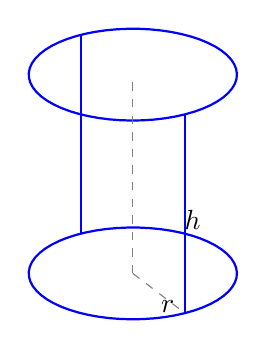
\begin{tikzpicture}
\begin{axis}[
    view={60}{30},
    axis lines=none,
    width=7cm, height=7cm,
    xmin=-1.5,xmax=1.5,
    ymin=-1.5,ymax=1.5,
    zmin=0,zmax=3
]
% Bottom ellipse
\addplot3[domain=0:360, samples=60, no marks, thick, blue]
    ({cos(x)},{sin(x)},{0});
% Top ellipse
\addplot3[domain=0:360, samples=60, no marks, thick, blue]
    ({cos(x)},{sin(x)},{2.5});
% Side lines
\addplot3[no marks, thick, blue] coordinates {(1,0,0) (1,0,2.5)};
\addplot3[no marks, thick, blue] coordinates {(-1,0,0) (-1,0,2.5)};
% Labels
\node at (axis cs:1.15,0,1.25) {$h$};
\node at (axis cs:0.5,0.1,0) [below] {$r$};
\addplot3[no marks, dashed, gray] coordinates {(0,0,0) (1,0,0)};
\addplot3[no marks, dashed, gray] coordinates {(0,0,0) (0,0,2.5)};
\end{axis}
\end{tikzpicture}
\caption{Stačiasis cilindras su spinduliu $r$ ir aukščiu $h$}
\end{figure}

\subsubsection*{Uždaviniai}

\begin{exercise}
Cilindro pagrindo spindulys $r = 3$ cm, aukštis $h = 5$ cm. Raskite cilindro tūrį ir viso paviršiaus plotą.

\textbf{Sprendimas:}
\begin{align*}
    V &= \pi r^2 h = \pi \cdot 9 \cdot 5 = 45\pi \approx 141{,}37 \text{ cm}^3 \\
    S_{\text{pav}} &= 2\pi r(h + r) = 2\pi \cdot 3 \cdot (5 + 3) = 48\pi \approx 150{,}80 \text{ cm}^2
\end{align*}
\end{exercise}

\begin{exercise}
Cilindro šoninis paviršiaus plotas $S_{\text{šon}} = 60\pi$ cm$^2$, aukštis $h = 10$ cm. Raskite cilindro spindulį ir tūrį.

\textbf{Sprendimas:}
\begin{align*}
    S_{\text{šon}} &= 2\pi r h \implies r = \frac{S_{\text{šon}}}{2\pi h} = \frac{60\pi}{2\pi \cdot 10} = 3 \text{ cm} \\
    V &= \pi r^2 h = \pi \cdot 9 \cdot 10 = 90\pi \approx 282{,}74 \text{ cm}^3
\end{align*}
\end{exercise}

\begin{exercise}[VBE tipo]
Į cilindrą, kurio pagrindo spindulys lygus $r$, įrašytas kubas. Raskite didžiausią galimą kubo kraštinės ilgį, jei cilindro aukštis $h = 2r$.

\textbf{Sprendimas:}

Kubo kraštinė $a$ yra įrašyta į apskritimą, todėl $a\sqrt{2} = 2r$, iš kur $a = r\sqrt{2}$.

Taip pat turi būti $a \leq h = 2r$, t.\,y. $r\sqrt{2} \leq 2r$ – tai teisinga. Todėl didžiausia kubo kraštinė $a = r\sqrt{2}$.
\end{exercise}

\begin{remark}
Cilindras gali būti laikomas prizmės ribine forma: kai taisyklingosios prizmės kraštinių skaičius $n \to \infty$, prizmė artėja į cilindrą.
\end{remark}

% ──────────────────────────────────────────────
\subsection{Kūgis}
% ──────────────────────────────────────────────

\begin{definition}
\textbf{Stačiasis kūgis} – sukimosi kūnas, gaunamas sukant stačiakampį trikampį aplink vieną iš jo statinių. Kūgis turi vieną apskritą pagrindą ir viršūnę (tašką).
\end{definition}

\subsubsection*{Pagrindiniai elementai}

\begin{itemize}
    \item $r$ – pagrindo apskritimo spindulys,
    \item $h$ – kūgio aukštis (atstumas nuo viršūnės iki pagrindo centro),
    \item $l$ – sudaromosios ilgis (atstumas nuo viršūnės iki pagrindo apskritimo taško),
    \item Ryšys tarp elementų: $l^2 = r^2 + h^2$ (Pitagoro teorema).
\end{itemize}

\subsubsection*{Formulės}

\begin{tcolorbox}[title=Kūgio formulės, colback=green!5!white, colframe=green!60!black]
\begin{align}
    l &= \sqrt{r^2 + h^2} \\
    S_{\text{šon}} &= \pi r l \\
    S_{\text{pav}} &= \pi r l + \pi r^2 = \pi r(l + r) \\
    V &= \frac{1}{3}\pi r^2 h
\end{align}
\end{tcolorbox}

\noindent Kūgio tūris yra \textbf{tris kartus mažesnis} už cilindro su tais pačiais $r$ ir $h$ tūrį.

\subsubsection*{Šoninio paviršiaus išskleidimas}

Kūgio šoninis paviršius išskleidžiamas į \textbf{skritulio išpjovą} su spinduliu $l$ (sudaromoji) ir lanko ilgiu $2\pi r$ (pagrindo apskritimo ilgis). Išpjovos kampas:
\[
    \alpha = \frac{2\pi r}{l} \text{ (radianais)} \quad \text{arba} \quad \alpha = \frac{360° \cdot r}{l}.
\]

\subsubsection*{Nupjautinis kūgis}

\begin{definition}
\textbf{Nupjautinis kūgis} gaunamas kūgio dalį nukirtus plokštuma, lygiagrečia pagrindui. Jo pagrindų spinduliai yra $r_1$ ir $r_2$ ($r_1 > r_2$), aukštis $h$, sudaromoji:
\[
    l = \sqrt{h^2 + (r_1 - r_2)^2}.
\]
\end{definition}

\begin{tcolorbox}[title=Nupjautinio kūgio formulės, colback=green!5!white, colframe=green!60!black]
\begin{align}
    S_{\text{šon}} &= \pi (r_1 + r_2)\, l \\
    V &= \frac{\pi h}{3}\left(r_1^2 + r_1 r_2 + r_2^2\right)
\end{align}
\end{tcolorbox}

\subsubsection*{Uždaviniai}

\begin{exercise}
Kūgio pagrindo spindulys $r = 4$ cm, aukštis $h = 3$ cm. Raskite sudaromosios ilgį, viso paviršiaus plotą ir tūrį.

\textbf{Sprendimas:}
\begin{align*}
    l &= \sqrt{r^2 + h^2} = \sqrt{16 + 9} = \sqrt{25} = 5 \text{ cm} \\
    S_{\text{pav}} &= \pi r(l + r) = \pi \cdot 4 \cdot (5 + 4) = 36\pi \approx 113{,}10 \text{ cm}^2 \\
    V &= \frac{1}{3}\pi r^2 h = \frac{1}{3}\pi \cdot 16 \cdot 3 = 16\pi \approx 50{,}27 \text{ cm}^3
\end{align*}
\end{exercise}

\begin{exercise}
Kūgio šoninis paviršiaus plotas lygus pagrindo plotui. Raskite kūgio pusviršūnkampį (kampą tarp aukštinės ir sudaromosios).

\textbf{Sprendimas:}

Sąlyga: $\pi r l = \pi r^2 \implies l = r$.

Pusviršūnkampis $\alpha$:
\[
    \sin\alpha = \frac{r}{l} = \frac{r}{r} = 1 \implies \alpha = 90°.
\]

Tai neįmanoma (kūgis „išsilygins"), todėl iš tikrųjų: $\cos\alpha = \frac{h}{l}$ ir $\sin\alpha = \frac{r}{l} = \frac{r}{r} = 1$ – kūgis virsta disku. Vadinasi, tokios sąlygos kūgis įvykdyti negali.
\end{exercise}

\begin{exercise}[VBE tipo]
Kūgio aukštis lygus $h$, o pusviršūnkampis $\alpha = 30°$. Raskite kūgio tūrį.

\textbf{Sprendimas:}

$\tg\,\alpha = \dfrac{r}{h} \implies r = h\tg\,30° = \dfrac{h}{\sqrt{3}}$

\[
V = \frac{1}{3}\pi r^2 h = \frac{1}{3}\pi \cdot \frac{h^2}{3} \cdot h = \frac{\pi h^3}{9}
\]
\end{exercise}

\begin{remark}
Kūgis gali būti laikomas piramidės ribine forma: kai taisyklingosios piramidės kraštinių skaičius $n \to \infty$, piramidė artėja į kūgį.
\end{remark}

% ──────────────────────────────────────────────
\subsection{Rutulys}
% ──────────────────────────────────────────────

\begin{definition}
\textbf{Rutulys} – tai erdvinė figūra, kurią riboja \textbf{sfera}: visi taškų, vienodai nutolusių atstumu $R$ nuo centro $O$, aibė. Rutulys gaunamas sukant pusapskritimį aplink jo skersmenį.
\end{definition}

\subsubsection*{Pagrindiniai elementai}

\begin{itemize}
    \item $R$ – rutulio spindulys (atstumas nuo centro iki sferos),
    \item $d = 2R$ – skersmuo,
    \item Didžiausias rutulio pjūvis plokštuma yra \textbf{didysis skritulys} su spinduliu $R$.
\end{itemize}

\subsubsection*{Formulės}

\begin{tcolorbox}[title=Rutulio formulės, colback=red!5!white, colframe=red!60!black]
\begin{align}
    S &= 4\pi R^2 \\
    V &= \frac{4}{3}\pi R^3
\end{align}
\end{tcolorbox}

\noindent Pastebėkite: rutulio paviršiaus plotas lygus \textbf{keturių didžiojo skritulio plotų} sumai ($4 \cdot \pi R^2$).

\subsubsection*{Rutulio nuopjova ir išpjova}

Kai rutulį kerta plokštuma, atsikerta \textbf{rutulio nuopjova} – sferos dalis aukštyje $h$.

\begin{tcolorbox}[title=Rutulio nuopjovos formulės, colback=red!5!white, colframe=red!60!black]
\begin{align}
    S_{\text{šon}} &= 2\pi R h \\
    V_{\text{nuopj}} &= \pi h^2\!\left(R - \frac{h}{3}\right)
\end{align}
\end{tcolorbox}

\noindent kur $h$ – nuopjovos aukštis, $R$ – rutulio spindulys.

\begin{remark}
Nuopjovos šoninio paviršiaus plotas $S = 2\pi Rh$ priklauso tik nuo $R$ ir $h$, bet nepriklauso nuo to, kurioje rutulio vietoje atliekamas pjūvis.
\end{remark}

\subsubsection*{Uždaviniai}

\begin{exercise}
Rutulio spindulys $R = 6$ cm. Raskite rutulio paviršiaus plotą ir tūrį.

\textbf{Sprendimas:}
\begin{align*}
    S &= 4\pi R^2 = 4\pi \cdot 36 = 144\pi \approx 452{,}39 \text{ cm}^2 \\
    V &= \frac{4}{3}\pi R^3 = \frac{4}{3}\pi \cdot 216 = 288\pi \approx 904{,}78 \text{ cm}^3
\end{align*}
\end{exercise}

\begin{exercise}
Rutulio paviršiaus plotas $S = 100\pi$ cm$^2$. Raskite rutulio spindulį ir tūrį.

\textbf{Sprendimas:}
\begin{align*}
    S = 4\pi R^2 &\implies R^2 = \frac{S}{4\pi} = \frac{100\pi}{4\pi} = 25 \implies R = 5 \text{ cm} \\
    V &= \frac{4}{3}\pi \cdot 125 = \frac{500\pi}{3} \approx 523{,}60 \text{ cm}^3
\end{align*}
\end{exercise}

\begin{exercise}[VBE tipo]
Į rutulį įrašytas cilindras. Cilindro aukštis $h = 2\sqrt{2}$ cm, o rutulio spindulys $R = 3$ cm. Raskite įrašytojo cilindro pagrindo spindulį $r$ ir cilindro tūrį.

\textbf{Sprendimas:}

Cilindro pagrindo spindulys ir rutulio spindulys susiję per Pitagoro teoremą:
\[
    r^2 + \left(\frac{h}{2}\right)^2 = R^2 \implies r^2 = R^2 - \frac{h^2}{4} = 9 - \frac{8}{4} = 9 - 2 = 7
\]
\[
    r = \sqrt{7} \text{ cm}, \quad V = \pi r^2 h = \pi \cdot 7 \cdot 2\sqrt{2} = 14\sqrt{2}\,\pi \approx 62{,}31 \text{ cm}^3
\]
\end{exercise}

\begin{exercise}[VBE tipo]
Į kūgį įrašytas rutulys. Kūgio aukštis $h = 4$ cm, pagrindo spindulys $r = 3$ cm. Raskite įrašytojo rutulio spindulį $\rho$.

\textbf{Sprendimas:}

Sudaromoji $l = \sqrt{r^2 + h^2} = \sqrt{9 + 16} = 5$ cm.

Kūgio skerspjūvis per ašį yra lygiašonis trikampis. Įrašytasis rutulys atitinka įrašytąjį apskritimą šiame trikampyje:
\[
    \rho = \frac{S_{\triangle}}{s}
\]
kur $S_{\triangle}$ – trikampio plotas, $s$ – pusis perimetro.
\[
    S_{\triangle} = \frac{1}{2} \cdot 2r \cdot h = \frac{1}{2} \cdot 6 \cdot 4 = 12 \text{ cm}^2
\]
\[
    s = \frac{2r + 2l}{2} = \frac{6 + 10}{2} = 8 \text{ cm}
\]
\[
    \rho = \frac{12}{8} = 1{,}5 \text{ cm}
\]
\end{exercise}

\subsubsection*{Sukimosi kūnų palyginimas}

\begin{table}[h]
\centering
\caption{Pagrindinių sukimosi kūnų formulių suvestinė}
\begin{tabular}{|l|c|c|c|}
\hline
\textbf{Kūnas} & \textbf{Šoninis plotas} & \textbf{Visas plotas} & \textbf{Tūris} \\
\hline
Cilindras & $2\pi r h$ & $2\pi r(r+h)$ & $\pi r^2 h$ \\
\hline
Kūgis & $\pi r l$ & $\pi r(r+l)$ & $\dfrac{1}{3}\pi r^2 h$ \\
\hline
Rutulys & — & $4\pi R^2$ & $\dfrac{4}{3}\pi R^3$ \\
\hline
\end{tabular}
\end{table}

\begin{remark}
Jei cilindras, kūgis ir rutulys turi vienodą pagrindo spindulį $r$ ir aukštį $h = 2r$, jų tūrių santykis yra:
\[
    V_{\text{kūgis}} : V_{\text{rutulio pusė}} : V_{\text{cilindras}} = 1 : 2 : 3.
\]
Šį ryšį atrado Archimedas ir laikė juo svarbiausiu savo gyvenimo atradimu.
\end{remark}


\section{Erdvinių kūnų pjūviai}

\subsection{Pjūvio sąvoka}

\begin{definition}
Erdvinio kūno \textbf{pjūvis} – tai plokštumos ir erdvinio kūno bendros dalies figūra, gaunama kertant kūną plokštuma. Pjūvio plokštuma vadinama \textbf{kertančiąja plokštuma}.
\end{definition}

Pjūvis visada yra plokščioji figūra (daugiakampis, apskritimas, elipsė ir pan.), kurios forma priklauso nuo to, kokiu kampu kertančioji plokštuma susikerta su kūnu. Pjūviai naudojami apskaičiuoti kūno savybes, sprendžiant inžinerines, architektūrines ir gamtos mokslų problemas.

\begin{remark}
Sprendžiant uždavinius svarbu:
\begin{enumerate}
    \item Teisingai identifikuoti pjūvio formą.
    \item Rasti pjūvio elemento ilgius, naudojantis Pitagoro teorema arba trigonometrinėmis formulėmis.
    \item Apskaičiuoti pjūvio plotą pagal atitinkamą plokštuminės figūros ploto formulę.
\end{enumerate}
\end{remark}

% -----------------------------------------------------------
\subsection{Briaunainių pjūviai}

Briaunainiai – tai daugiakampiais apriboti erdviniai kūnai (prizmės, piramidės, kubas ir kt.). Jų pjūviai yra daugiakampiai.

\subsubsection{Kubo pjūviai}

Tegu kubas turi kraštinę $a$. Priklausomai nuo kertančiosios plokštumos padėties, galimi šie pjūviai:

\begin{itemize}
    \item \textbf{Kvadratas} – plokštuma statmena kraštinei ir lygiagreti vienai iš sienų.
    \item \textbf{Stačiakampis} – plokštuma lygiagreti dviem priešingoms briaunoms, bet ne sienoms.
    \item \textbf{Trikampis} – plokštuma kerta tris briaunas, praeinančias per vieną viršūnę.
    \item \textbf{Taisyklingasis šešiakampis} – plokštuma statmena kubo erdvinei įstrižainei ir praeina per jos vidurį.
\end{itemize}

\begin{example}
Kubo $ABCDA_1B_1C_1D_1$ kraštinė lygi $a$. Plokštuma kerta kubą per viršūnes $B_1$, $D$ ir briaunų $AB$, $D_1C_1$ vidurio taškus $P$ ir $K$. Raskite pjūvio plotą.

\textbf{Sprendimas.}

Pjūvio figūra – rombas $PB_1KD$.
\begin{align*}
PK &= \sqrt{a^2 + a^2} = a\sqrt{2} \quad \text{(šoninės sienos įstrižainė)},\\
B_1D &= \sqrt{a^2 + a^2 + a^2} = a\sqrt{3} \quad \text{(erdvinė kubo įstrižainė)}.
\end{align*}
Rombo plotas:
\[
S = \frac{1}{2} \cdot d_1 \cdot d_2 = \frac{1}{2} \cdot a\sqrt{2} \cdot a\sqrt{3} = \frac{a^2\sqrt{6}}{2}.
\]
\end{example}

% -----------------------------------------------------------
\subsubsection{Prizmės pjūviai}

\begin{definition}
\textbf{Statmenas pjūvis} – pjūvis, gautas kertant prizmę plokštuma, statmena šoninėms briaunoms.\\
\textbf{Įstrižinis pjūvis} – pjūvis, gautas kertant prizmę plokštuma, einančia per dvi vienoje sienoje nesančias šonines briaunas.
\end{definition}

Taisyklingosios $n$-kampės prizmės, kurios pagrindo kraštinė $a$, aukštis $h$:

\begin{itemize}
    \item \textbf{Pjūvis lygiagretus pagrindui} – taisyklingasis $n$-kampis, lygus pagrindui.
    \item \textbf{Statmenas pjūvis} – taisyklingasis $n$-kampis su apotema $r$ (vidinė apskritimo spindulys).
    \item \textbf{Stačiakampės prizmės įstrižinis pjūvis} – stačiakampis, kurio kraštinės $a$ ir $d$, kur $d$ – pjūvio įstrižainė.
\end{itemize}

\begin{example}
Taisyklingosios keturkampės prizmės pagrindo kraštinė $a = 6$ cm, aukštis $h = 8$ cm. Raskite įstrižinio pjūvio (kertančio per pagrindo įstrižainę) plotą.

\textbf{Sprendimas.}

Pagrindo įstrižainė:
\[
d_{\text{pagr}} = a\sqrt{2} = 6\sqrt{2} \text{ cm}.
\]
Pjūvis yra stačiakampis su kraštinėmis $d_{\text{pagr}}$ ir $h$:
\[
S = d_{\text{pagr}} \cdot h = 6\sqrt{2} \cdot 8 = 48\sqrt{2} \approx 67{,}88 \text{ cm}^2.
\]
\end{example}

% -----------------------------------------------------------
\subsubsection{Piramidės pjūviai}

Taisyklingosios $n$-kampės piramidės pjūviai:

\begin{itemize}
    \item \textbf{Pjūvis lygiagretus pagrindui} – taisyklingasis $n$-kampis, panašus į pagrindą. Jei pjūvis nutolęs nuo viršūnės atstumu $h'$, o piramidės aukštis $H$, tai pjūvio kraštinė:
    \[
    a' = a \cdot \frac{h'}{H},
    \]
    o pjūvio plotas:
    \[
    S_{\text{pjūvio}} = S_{\text{pagr}} \cdot \left(\frac{h'}{H}\right)^2.
    \]
    \item \textbf{Įstrižinis (ašinis) pjūvis} – trikampis, einantis per viršūnę ir pagrindo įstrižainę (arba kraštinę).
\end{itemize}

\begin{example}
Taisyklingosios keturkampės piramidės $SABCD$ pagrindo kraštinė $a = 20$ cm, aukštis $H = 20$ cm. Raskite:
\begin{enumerate}[label=\alph*)]
    \item įstrižinio pjūvio $SAC$ plotą,
    \item pjūvio, lygiagrečio pagrindui ir nutolusio nuo jo $10$ cm, plotą.
\end{enumerate}

\textbf{Sprendimas.}

\textbf{a)} Pagrindo $ABCD$ įstrižainė:
\[
AC = a\sqrt{2} = 20\sqrt{2} \text{ cm}.
\]
Piramidės aukštinė $SO = H = 20$ cm (krenta į pagrindo centrą $O$). Trikampio $SAC$ plotas:
\[
S_{\triangle SAC} = \frac{1}{2} \cdot AC \cdot SO = \frac{1}{2} \cdot 20\sqrt{2} \cdot 20 = 200\sqrt{2} \approx 282{,}84 \text{ cm}^2.
\]

\textbf{b)} Pjūvis nutolęs nuo pagrindo $10$ cm, vadinasi nuo viršūnės nutolęs $H - 10 = 10$ cm. Taigi $h' = 10$ cm, $H = 20$ cm.
\[
S_{\text{pjūvio}} = S_{\text{pagr}} \cdot \left(\frac{h'}{H}\right)^2 = (20)^2 \cdot \left(\frac{10}{20}\right)^2 = 400 \cdot \frac{1}{4} = 100 \text{ cm}^2.
\]
\end{example}

% -----------------------------------------------------------
\subsection{Sukinių pjūviai}

Sukiniai – tai kūnai, gauti sukant plokščiąją figūrą aplink tiesę (ašį). Pagrindiniai sukiniai: cilindras, kūgis, rutulys.

\subsubsection{Cilindro pjūviai}

Tiesaus apskritiminio cilindro, kurio pagrindo spindulys $r$ ir aukštis $h$:

\begin{itemize}
    \item \textbf{Pjūvis lygiagretus pagrindui} – apskritimas, kurio spindulys $r$ ir plotas $S = \pi r^2$.
    \item \textbf{Ašinis pjūvis} (plokštuma eina per ašį) – stačiakampis $2r \times h$, kurio plotas:
    \[
    S_{\text{ašinis}} = 2r \cdot h.
    \]
    \item \textbf{Pjūvis statmenas ašiai} – apskritimas, kurio spindulys $r$.
    \item \textbf{Įstrižinis pjūvis} (plokštuma kerta abi pagrindų apskritimus) – elipsė.
\end{itemize}

\begin{example}
Cilindro pagrindo spindulys $r = 5$ cm, aukštis $h = 12$ cm. Raskite ašinio pjūvio plotą ir perimetrą.

\textbf{Sprendimas.}

Ašinis pjūvis yra stačiakampis, kurio kraštinės $2r = 10$ cm ir $h = 12$ cm.
\[
S = 2r \cdot h = 10 \cdot 12 = 120 \text{ cm}^2.
\]
\[
P = 2(2r + h) = 2(10 + 12) = 44 \text{ cm}.
\]
\end{example}

% -----------------------------------------------------------
\subsubsection{Kūgio pjūviai}

Tiesaus apskritiminio kūgio, kurio pagrindo spindulys $r$, aukštis $h$, sudaromoji $l = \sqrt{r^2 + h^2}$:

\begin{itemize}
    \item \textbf{Pjūvis lygiagretus pagrindui}, nutolęs nuo viršūnės atstumu $h'$: apskritimas, kurio spindulys
    \[
    r' = r \cdot \frac{h'}{h}.
    \]
    \item \textbf{Ašinis pjūvis} – lygiašonis trikampis, kurio pagrindas $2r$ ir šonai $l$. Plotas:
    \[
    S_{\text{ašinis}} = \frac{1}{2} \cdot 2r \cdot h = r \cdot h.
    \]
    \item \textbf{Pjūvis per dvi sudaromąsias} – lygiašonis trikampis su ta pačia ašinio pjūvio forma.
    \item \textbf{Įstrižinis pjūvis} (plokštuma kerta pagrindo apskritimą, bet neina per ašį) – elipsė arba parabolė (atskirais atvejais).
\end{itemize}

\begin{example}
Kūgio sudaromoji $l = 12$ cm, pagrindo spindulys $r = 6$ cm. Plokštuma eina per dvi sudaromąsias $AB$ ir $AC$, kurios sudaro kampą $60°$. Raskite pjūvio plotą ir kampą tarp pjūvio ir kūgio pagrindo.

\textbf{Sprendimas.}

Pjūvis – trikampis $ABC$, kur $AB = AC = l = 12$ cm ir $\angle BAC = 60°$. Trikampis yra lygiašonis su viršūniniu kampu $60°$, vadinasi lygiakraštis:
\[
BC = AB = AC = 12 \text{ cm}.
\]
Trikampio plotas:
\[
S = \frac{\sqrt{3}}{4} \cdot 12^2 = \frac{\sqrt{3}}{4} \cdot 144 = 36\sqrt{3} \approx 62{,}35 \text{ cm}^2.
\]
Aukštinė $h = \sqrt{l^2 - r^2} = \sqrt{144 - 36} = \sqrt{108} = 6\sqrt{3}$ cm.
Pjūvio vidurio taškas nuo pagrindo centro: trikampio pjūvio aukštinė $SO = 6\sqrt{3}$ cm. Trijų statmenų teorema leidžia rasti kampą $\varphi$ tarp pjūvio plokštumos ir pagrindo:
\[
\tg\varphi = \frac{h}{r} = \frac{6\sqrt{3}}{6} = \sqrt{3} \implies \varphi = 60°.
\]
\end{example}

% -----------------------------------------------------------
\subsubsection{Rutulio pjūviai}

\begin{definition}
Rutulio, kurio spindulys $R$, bet kuris pjūvis yra \textbf{apskritimas}. Jei kertančioji plokštuma nutolusi nuo centro atstumu $d$ ($0 \leq d < R$), tai pjūvio apskritimo spindulys:
\[
\rho = \sqrt{R^2 - d^2}.
\]
\end{definition}

\begin{itemize}
    \item Kai $d = 0$ (plokštuma eina per centrą), gaunamas \textbf{didysis apskritimas}, kurio spindulys $\rho = R$ ir plotas $S = \pi R^2$.
    \item Kai $d \to R$, pjūvio spindulys $\rho \to 0$ (taškas).
    \item Pjūvio plotas:
    \[
    S_{\text{pjūvio}} = \pi \rho^2 = \pi(R^2 - d^2).
    \]
\end{itemize}

\begin{example}
Rutulio spindulys $R = 10$ cm. Plokštuma nutolusi nuo rutulio centro 6 cm. Raskite pjūvio plotą.

\textbf{Sprendimas.}
\[
\rho = \sqrt{R^2 - d^2} = \sqrt{100 - 36} = \sqrt{64} = 8 \text{ cm}.
\]
\[
S = \pi\rho^2 = 64\pi \approx 201{,}06 \text{ cm}^2.
\]
\end{example}

% -----------------------------------------------------------
\subsection{Trijų statmenų teorema ir pjūviai}

Nustatant kampo tarp pjūvio plokštumos ir kūno pagrindo dydį, dažnai taikoma \textbf{trijų statmenų teorema}.

\begin{theorem}[Trijų statmenų teorema]
Jei tiesė $MN$ guli plokštumoje $\alpha$, tiesė $PQ$ yra statmena plokštumai $\alpha$ ir $PQ \perp MN$, tai tiesė $MN$ yra statmena ir projekcijai $M'N'$ plokštumoje $\beta$.
\end{theorem}

\begin{remark}
Atvirkštinė teorema taip pat galioja: jei tiesė yra statmena jos projekcijai kitoje plokštumoje, tai ji statmena ir pačiai plokštumai.
\end{remark}

\begin{example}
Taisyklingosios trikampės piramidės pagrindo kraštinė $a$, aukštis $H$. Raskite kampą tarp šoninės sienos ir pagrindo.

\textbf{Sprendimas.}

Šoninės sienos apotema (aukštinė):
\[
l_{\text{ap}} = \sqrt{H^2 + r_{\text{vid}}^2}, \quad r_{\text{vid}} = \frac{a}{2\sqrt{3}}.
\]
Kampas $\varphi$ tarp šoninės sienos ir pagrindo:
\[
\tg\varphi = \frac{H}{r_{\text{vid}}} = \frac{H}{\dfrac{a}{2\sqrt{3}}} = \frac{2H\sqrt{3}}{a}.
\]
\end{example}

% -----------------------------------------------------------
\subsection{Pjūvių formos suvestinė}

\begin{center}
\begin{tabular}{|l|l|l|}
\hline
\textbf{Kūnas} & \textbf{Pjūvio kryptis} & \textbf{Pjūvio forma} \\
\hline
Kubas & Lygiagrečiai sienai & Kvadratas \\
Kubas & Per ašį ir dvi briaunas & Stačiakampis \\
Kubas & Per tris viršūnes & Trikampis \\
Kubas & Statmenai erdvinei įstrižainei & Taisyklingasis šešiakampis \\
\hline
Prizmė & Lygiagrečiai pagrindui & Pagrindo forma \\
Prizmė & Statmenai šoninėms briaunoms & Pagrindo forma \\
Prizmė & Per dvi šonines briaunas & Daugiakampis \\
\hline
Piramidė & Lygiagrečiai pagrindui & Panašus į pagrindą \\
Piramidė & Per viršūnę ir pagrindo įstrižainę & Trikampis \\
\hline
Cilindras & Lygiagrečiai pagrindui & Apskritimas \\
Cilindras & Per ašį & Stačiakampis \\
Cilindras & Įstrižai & Elipsė \\
\hline
Kūgis & Lygiagrečiai pagrindui & Apskritimas \\
Kūgis & Per ašį & Lygiašonis trikampis \\
Kūgis & Įstrižai (nekertant pagrindo) & Elipsė / Parabolė \\
\hline
Rutulys & Bet kokia kryptis & Apskritimas \\
\hline
\end{tabular}
\end{center}

% -----------------------------------------------------------
\subsection{VBE tipo uždaviniai}

\begin{exercise}
Taisyklingosios šešiakampės prizmės pagrindo kraštinė $a = 4$ cm, aukštis $h = 6$ cm. Plokštuma kerta prizmę per vieną pagrindo kraštinę ir priešingos šoninės sienos vidurinę liniją. Raskite pjūvio perimetrą ir plotą.
\end{exercise}

\begin{exercise}
Kūgio aukštis $h = 8$ cm, pagrindo spindulys $r = 6$ cm. Raskite pjūvio, lygiagrečio pagrindui ir nutolusio nuo pagrindo $4$ cm atstumu, plotą.
\end{exercise}

\begin{exercise}
Rutulio didžiojo apskritimo ilgis $C = 10\pi$ cm. Plokštuma nutolusi nuo rutulio centro $3$ cm. Raskite pjūvio plotą.
\end{exercise}

\begin{exercise}
Stačiakampės prizmės pagrindo kraštinės $a = 5$ cm ir $b = 12$ cm, aukštis $h = 8$ cm. Plokštuma eina per ilgąją pagrindo kraštinę $b$ ir priešingos šoninės sienos viršutinę briauną. Raskite pjūvio plotą ir kampą tarp pjūvio plokštumos ir prizmės pagrindo.
\end{exercise}

\begin{exercise}
Taisyklingosios keturkampės piramidės kraštinė $a = 10$ cm ir aukštis $H = 12$ cm. Plokštuma lygiagreti pagrindui ir dalija piramidę į dvi lygaus tūrio dalis. Raskite pjūvio plotą.
\end{exercise}


\section{Paviršiaus plotas ir tūris}

Erdvinių figūrų matavimas yra viena iš svarbiausių matematikos VBE temų. Šiame skyriuje nagrinėsime, kaip apskaičiuoti daugiasienių bei sukimosi kūnų paviršiaus plotus ir tūrius, remdamiesi oficialaus egzamino formulių rinkinio formulėmis.

% ============================================================
\subsection{Daugiasienių paviršius ir tūris}
% ============================================================

\begin{definition}
\textbf{Daugiasienė} (arba \textbf{daugiakampis kūnas}) -- erdvinė figūra, kurios paviršių sudaro baigtinis skaičius plokštuminių daugiakampių (sienų). Kiekvienos sienos kraštinės vadinamos \emph{briaunomis}, o briaunų susikirtimo taškai -- \emph{viršūnėmis}.
\end{definition}

\begin{definition}
\textbf{Paviršiaus plotas} $S$ -- tai visų kūno sienų plotų suma. \textbf{Tūris} $V$ -- tai kūno užimamo erdvės dydis.
\end{definition}

% -------------------------------------------------------
\subsubsection*{Stačiakampis gretasienis ir kubas}
% -------------------------------------------------------

\begin{definition}
\textbf{Stačiakampis gretasienis} -- tai šešiasienė, kurios visos sienos yra stačiakampiai. Jo matmenys žymimi: ilgis~$a$, plotis~$b$, aukštis~$c$.
\end{definition}

\begin{theorem}
Stačiakampio gretasienio, kurio briaunų ilgiai yra $a$, $b$ ir $c$, paviršiaus plotas ir tūris:
\[
S = 2(ab + bc + ca), \qquad V = abc.
\]
\end{theorem}

\begin{remark}
\textbf{Kubas} -- tai ypatinga gretasienio forma, kai $a = b = c$. Todėl:
\[
S_{\text{kubo}} = 6a^2, \qquad V_{\text{kubo}} = a^3.
\]
\end{remark}

\begin{example}
Stačiakampio gretasienio matmenys: $a = 5$~cm, $b = 3$~cm, $c = 4$~cm. Raskite jo paviršiaus plotą ir tūrį.

\textbf{Sprendimas:}
\[
S = 2(5 \cdot 3 + 3 \cdot 4 + 4 \cdot 5) = 2(15 + 12 + 20) = 2 \cdot 47 = 94 \text{ cm}^2.
\]
\[
V = 5 \cdot 3 \cdot 4 = 60 \text{ cm}^3.
\]
\end{example}

% -------------------------------------------------------
\subsubsection*{Prizmė}
% -------------------------------------------------------

\begin{definition}
\textbf{Prizmė} -- tai daugiasienė, kurios du pagrindai yra lygiagrečiose plokštumose esantys vienodi daugiakampiai, o šoninės sienos yra lygiagretainiai.
\begin{itemize}
    \item \textbf{Tiesiosios prizmės} šoninės briaunos yra statmenos pagrindų plokštumoms.
    \item \textbf{Taisyklingosios prizmės} pagrindai yra taisyklingi daugiakampiai, o pati prizmė yra tiesiosios.
\end{itemize}
\end{definition}

\begin{theorem}[Prizmės paviršius ir tūris]
Tiesiosios prizmės, kurios pagrindo perimetras $P$, pagrindo plotas $S_{\text{pagr}}$ ir aukštinės ilgis $H$:
\[
S_{\text{šon}} = P \cdot H, \qquad S = S_{\text{šon}} + 2S_{\text{pagr}}, \qquad V = S_{\text{pagr}} \cdot H.
\]
\end{theorem}

\begin{remark}
Taisyklingosios $n$-kampės prizmės pagrindas yra taisyklingasis $n$-kampis, kurio kraštinės ilgis $a$. Šio pagrindo plotas:
\[
S_{\text{pagr}} = \frac{n \cdot a^2}{4} \ctg\frac{\pi}{n}.
\]
Dažniausiai egzamine sutinkamos taisyklingosios trikampė, keturkampė ir šešiakampė prizmės.
\end{remark}

\begin{example}
Taisyklingoji keturkampė prizmė (stačiakampė prizmė su kvadrato pagrindu) turi pagrindo kraštinę $a = 6$~cm ir aukštinę $H = 10$~cm. Raskite šoninį paviršiaus plotą, visą paviršiaus plotą ir tūrį.

\textbf{Sprendimas:}
\begin{align*}
S_{\text{pagr}} &= 6^2 = 36 \text{ cm}^2,\\
P &= 4 \cdot 6 = 24 \text{ cm},\\
S_{\text{šon}} &= 24 \cdot 10 = 240 \text{ cm}^2,\\
S &= 240 + 2 \cdot 36 = 312 \text{ cm}^2,\\
V &= 36 \cdot 10 = 360 \text{ cm}^3.
\end{align*}
\end{example}

\begin{example}
Taisyklingoji trikampė prizmė turi pagrindo kraštinę $a = 4$~cm ir aukštinę $H = 9$~cm. Apskaičiuokite jos tūrį.

\textbf{Sprendimas:} Taisyklingojo trikampio, kurio kraštinė $a$, plotas:
\[
S_{\text{pagr}} = \frac{a^2\sqrt{3}}{4} = \frac{16\sqrt{3}}{4} = 4\sqrt{3} \text{ cm}^2.
\]
\[
V = S_{\text{pagr}} \cdot H = 4\sqrt{3} \cdot 9 = 36\sqrt{3} \approx 62{,}35 \text{ cm}^3.
\]
\end{example}

% -------------------------------------------------------
\subsubsection*{Piramidė}
% -------------------------------------------------------

\begin{definition}
\textbf{Piramidė} -- tai daugiasienė, kurios pagrindas yra daugiakampis, o visos šoninės sienos yra trikampiai, turintys bendrą viršūnę (vadinamą \emph{piramidės viršūne}).

\textbf{Taisyklingoji piramidė} -- tai piramidė, kurios pagrindas yra taisyklingasis daugiakampis, o aukštinė eina per pagrindo centrą. Taisyklingosios piramidės šoninės sienos yra vienodi lygiašoniai trikampiai. Šoninių trikampių aukštinės (einančios iš piramidės viršūnės į pagrindo kraštinių vidurius) vadinamos \emph{apotema} ir žymimos $h$.
\end{definition}

\begin{theorem}[Piramidės paviršius ir tūris]
Piramidės, kurios pagrindo plotas $S_{\text{pagr}}$ ir aukštinė $H$, tūris:
\[
V = \frac{1}{3} S_{\text{pagr}} \cdot H.
\]
Taisyklingosios piramidės šoninis paviršiaus plotas:
\[
S_{\text{šon}} = \frac{1}{2} P \cdot h,
\]
čia $P$ -- pagrindo perimetras, $h$ -- apotema. Visas paviršiaus plotas:
\[
S = S_{\text{šon}} + S_{\text{pagr}}.
\]
\end{theorem}

\begin{remark}
Apotemos $h$, aukštinės $H$ ir pagrindo apotemos $r$ (įbrėžtinio apskritimo spindulys) ryšys:
\[
h^2 = H^2 + r^2.
\]
Šoninės briaunos $l$, aukštinės $H$ ir pagrindo apibrėžtinio apskritimo spindulio $R$ ryšys:
\[
l^2 = H^2 + R^2.
\]
\end{remark}

\begin{example}
Taisyklingoji keturkampė piramidė turi pagrindo kraštinę $a = 6$~cm ir aukštinę $H = 4$~cm. Raskite apofemą, šoninį paviršiaus plotą ir tūrį.

\textbf{Sprendimas:} Kvadrato įbrėžtinio apskritimo spindulys: $r = a/2 = 3$~cm.
\[
h = \sqrt{H^2 + r^2} = \sqrt{16 + 9} = \sqrt{25} = 5 \text{ cm}.
\]
\[
P = 4 \cdot 6 = 24 \text{ cm}, \quad S_{\text{šon}} = \frac{1}{2} \cdot 24 \cdot 5 = 60 \text{ cm}^2.
\]
\[
S_{\text{pagr}} = 6^2 = 36 \text{ cm}^2, \quad S = 60 + 36 = 96 \text{ cm}^2.
\]
\[
V = \frac{1}{3} \cdot 36 \cdot 4 = 48 \text{ cm}^3.
\]
\end{example}

% -------------------------------------------------------
\subsubsection*{Nupjautinė piramidė}
% -------------------------------------------------------

\begin{definition}
\textbf{Nupjautinė piramidė} -- tai kūnas, gaunamas, kai iš piramidės atpjaunamas viršūninis gabalas plokštuma, lygiagrečia pagrindui. Jos pagrindai yra du panašūs daugiakampiai, kurių plotai $S_1$ (didesnysis) ir $S_2$ (mažesnysis), o aukštinė $H$.
\end{definition}

\begin{theorem}[Nupjautinės piramidės tūris]
\[
V = \frac{H}{3}\left(S_1 + \sqrt{S_1 S_2} + S_2\right).
\]
\end{theorem}

\begin{theorem}[Taisyklingosios nupjautinės piramidės šoninis paviršius]
\[
S_{\text{šon}} = \frac{1}{2}(P_1 + P_2) \cdot h,
\]
čia $P_1$ ir $P_2$ -- pagrindų perimetrai, $h$ -- šoninių trapecijų aukštinė (apotema).
\end{theorem}

\begin{example}
Taisyklingoji keturkampė nupjautinė piramidė turi apatinį pagrindą $a_1 = 8$~cm, viršutinį pagrindą $a_2 = 4$~cm ir aukštinę $H = 6$~cm. Raskite jos tūrį.

\textbf{Sprendimas:}
\[
S_1 = 8^2 = 64 \text{ cm}^2, \quad S_2 = 4^2 = 16 \text{ cm}^2, \quad \sqrt{S_1 S_2} = \sqrt{64 \cdot 16} = \sqrt{1024} = 32 \text{ cm}^2.
\]
\[
V = \frac{6}{3}(64 + 32 + 16) = 2 \cdot 112 = 224 \text{ cm}^3.
\]
\end{example}

% -------------------------------------------------------
\subsubsection*{Uždaviniai}
% -------------------------------------------------------

\begin{exercise}
Taisyklingosios trikampės prizmės pagrindo kraštinė lygi $a$, o šoninės briaunos ilgis lygus $a$. Išreikškite prizmės tūrį ir paviršiaus plotą per $a$.
\end{exercise}

\begin{exercise}
Taisyklingoji šešiakampė piramidė turi pagrindo kraštinę $6$~cm ir šoninės briaunos ilgį $10$~cm. Raskite piramidės tūrį ir visą paviršiaus plotą.
\end{exercise}

\begin{exercise}
Kubo tūris lygus $216$~cm$^3$. Raskite kubo paviršiaus plotą ir erdvines įstrižaines ilgį.
\end{exercise}

\begin{exercise}
Stačiakampio gretasienio matmenų santykis $a : b : c = 1 : 2 : 3$. Paviršiaus plotas lygus $88$~cm$^2$. Raskite gretasienio tūrį.
\end{exercise}

% ============================================================
\subsection{Sukimosi kūnų paviršius ir tūris}
% ============================================================

\begin{definition}
\textbf{Sukimosi kūnas} -- tai erdvinė figūra, gaunama sukant plokštuminę figūrą apie ašį, kuri yra toje pačioje plokštumoje. Pagrindiniai sukimosi kūnai yra \emph{cilindras}, \emph{kūgis} ir \emph{rutulys}.
\end{definition}

% -------------------------------------------------------
\subsubsection*{Cilindras}
% -------------------------------------------------------

\begin{definition}
\textbf{Cilindras} -- tai sukimosi kūnas, gaunamas sukant stačiakampį aplink vieną jo kraštinę. Cilindro pagrindai yra du lygiagrečiuose plokštumuose esantys vienodi skrituliai, kurių spindulys $R$. Cilindro aukštinė $H$ yra atkarpa, jungianti pagrindų centrus ir statmena pagrindų plokštumoms.
\end{definition}

\begin{theorem}[Cilindro paviršius ir tūris]
\[
S_{\text{šon}} = 2\pi R H, \qquad S = 2\pi R H + 2\pi R^2 = 2\pi R(H + R),
\]
\[
V = \pi R^2 H.
\]
\end{theorem}

\begin{remark}
Cilindro šoninis paviršius, išvyniotas į plokštumą, tampa stačiakampiu, kurio ilgis lygus pagrindo apskritimo ilgiui $2\pi R$, o plotis -- aukštinei $H$.
\end{remark}

\begin{example}
Cilindro pagrindo spindulys $R = 5$~cm, aukštinė $H = 12$~cm. Raskite šoninį paviršiaus plotą, visą paviršiaus plotą ir tūrį.

\textbf{Sprendimas:}
\[
S_{\text{šon}} = 2\pi \cdot 5 \cdot 12 = 120\pi \approx 376{,}99 \text{ cm}^2.
\]
\[
S = 2\pi \cdot 5(12 + 5) = 10\pi \cdot 17 = 170\pi \approx 534{,}07 \text{ cm}^2.
\]
\[
V = \pi \cdot 25 \cdot 12 = 300\pi \approx 942{,}48 \text{ cm}^3.
\]
\end{example}

% -------------------------------------------------------
\subsubsection*{Kūgis}
% -------------------------------------------------------

\begin{definition}
\textbf{Kūgis} -- tai sukimosi kūnas, gaunamas sukant stačiakampį trikampį aplink vieną jo statinį. Kūgio pagrindas yra skritulys, kurio spindulys $R$. Kūgio aukštinė $H$ -- tai atkarpa nuo viršūnės iki pagrindo centro, statmena pagrindui. \textbf{Sudaromoji} $l$ -- tai atkarpa nuo viršūnės iki pagrindo apskritimo taško:
\[
l = \sqrt{H^2 + R^2}.
\]
\end{definition}

\begin{theorem}[Kūgio paviršius ir tūris]
\[
S_{\text{šon}} = \pi R l, \qquad S = \pi R l + \pi R^2 = \pi R(l + R),
\]
\[
V = \frac{1}{3}\pi R^2 H.
\]
\end{theorem}

\begin{remark}
Kūgio šoninis paviršius, išvyniotas į plokštumą, yra skritulio išpjova (sektorius), kurio spindulys lygus sudaromajai $l$, o lanko ilgis -- $2\pi R$.
\end{remark}

\begin{example}
Kūgio pagrindo spindulys $R = 3$~cm, aukštinė $H = 4$~cm. Raskite sudaromąją, šoninį paviršiaus plotą ir tūrį.

\textbf{Sprendimas:}
\[
l = \sqrt{H^2 + R^2} = \sqrt{16 + 9} = \sqrt{25} = 5 \text{ cm}.
\]
\[
S_{\text{šon}} = \pi \cdot 3 \cdot 5 = 15\pi \approx 47{,}12 \text{ cm}^2.
\]
\[
S = \pi \cdot 3(5 + 3) = 24\pi \approx 75{,}40 \text{ cm}^2.
\]
\[
V = \frac{1}{3}\pi \cdot 9 \cdot 4 = 12\pi \approx 37{,}70 \text{ cm}^3.
\]
\end{example}

% -------------------------------------------------------
\subsubsection*{Nupjautinis kūgis}
% -------------------------------------------------------

\begin{definition}
\textbf{Nupjautinis kūgis} -- tai kūnas, gaunamas, kai iš kūgio atpjaunamas viršūninis gabalas plokštuma, lygiagrečia pagrindui. Jo pagrindų spinduliai $R$ (didesnysis) ir $r$ (mažesnysis), aukštinė $H$, o sudaromoji:
\[
l = \sqrt{H^2 + (R - r)^2}.
\]
\end{definition}

\begin{theorem}[Nupjautinio kūgio paviršius ir tūris]
\[
S_{\text{šon}} = \pi(R + r)l, \qquad S = \pi(R + r)l + \pi R^2 + \pi r^2,
\]
\[
V = \frac{\pi H}{3}(R^2 + Rr + r^2).
\]
\end{theorem}

\begin{example}
Nupjautinio kūgio pagrindų spinduliai $R = 6$~cm ir $r = 3$~cm, aukštinė $H = 4$~cm. Raskite jo tūrį ir šoninį paviršiaus plotą.

\textbf{Sprendimas:}
\[
l = \sqrt{4^2 + (6-3)^2} = \sqrt{16 + 9} = 5 \text{ cm}.
\]
\[
S_{\text{šon}} = \pi(6 + 3) \cdot 5 = 45\pi \approx 141{,}37 \text{ cm}^2.
\]
\[
V = \frac{\pi \cdot 4}{3}(36 + 18 + 9) = \frac{4\pi}{3} \cdot 63 = 84\pi \approx 263{,}89 \text{ cm}^3.
\]
\end{example}

% -------------------------------------------------------
\subsubsection*{Rutulys}
% -------------------------------------------------------

\begin{definition}
\textbf{Rutulys} -- tai erdvinė figūra, kurią sudaro visi taškai, kurių atstumas nuo duoto taško (centro) neviršija $R$ (spindulio). \textbf{Sfera} -- tai visi taškai, kurių atstumas nuo centro lygiai lygus $R$ (rutulio paviršius).
\end{definition}

\begin{theorem}[Rutulio paviršius ir tūris]
\[
S = 4\pi R^2, \qquad V = \frac{4}{3}\pi R^3.
\]
\end{theorem}

\begin{remark}
Pastebėkite elegantišką ryšį tarp rutulio tūrio ir paviršiaus:
\[
V = \frac{R \cdot S}{3}.
\]
Tai analogiška piramidės tūrio formulei $V = \frac{1}{3}S_{\text{pagr}} \cdot H$.
\end{remark}

\begin{example}
Rutulio spindulys $R = 6$~cm. Raskite rutulio paviršiaus plotą ir tūrį.

\textbf{Sprendimas:}
\[
S = 4\pi \cdot 36 = 144\pi \approx 452{,}39 \text{ cm}^2.
\]
\[
V = \frac{4}{3}\pi \cdot 216 = 288\pi \approx 904{,}78 \text{ cm}^3.
\]
\end{example}

\begin{example}
Rutulio paviršiaus plotas $S = 100\pi$~cm$^2$. Raskite rutulio spindulį ir tūrį.

\textbf{Sprendimas:}
\[
4\pi R^2 = 100\pi \implies R^2 = 25 \implies R = 5 \text{ cm}.
\]
\[
V = \frac{4}{3}\pi \cdot 5^3 = \frac{500\pi}{3} \approx 523{,}60 \text{ cm}^3.
\]
\end{example}

% -------------------------------------------------------
\subsubsection*{Rutulio išpjova (kepurėlė)}
% -------------------------------------------------------

\begin{definition}
\textbf{Rutulio kepurėlė} (išpjova) -- tai dalis rutulio, atkertama plokštuma. Kepurėlės aukštinė $H$ -- tai didžiausias atstumas nuo atkirtos plokštumos iki rutulio paviršiaus. Rutulio spindulys $R$, kepurėlės pagrindo skritulys turi spindulį $r = \sqrt{R^2 - (R-H)^2} = \sqrt{2RH - H^2}$.
\end{definition}

\begin{theorem}[Rutulio kepurėlės paviršius ir tūris]
\[
S_{\text{šon}} = 2\pi R H, \qquad V = \frac{\pi H^2}{3}(3R - H).
\]
\end{theorem}

\begin{remark}
Svarbu atskirti: kepurėlės šoninis paviršius $2\pi RH$ priklauso tik nuo rutulio spindulio ir kepurėlės aukštinės, o ne nuo pagrindo spindulio.
\end{remark}

% -------------------------------------------------------
\subsubsection*{Formulių suvestinė}
% -------------------------------------------------------

\begin{tcolorbox}[title={Sukimosi kūnų formulių lentelė}, colback=blue!5, colframe=blue!50!black]
\begin{center}
\renewcommand{\arraystretch}{1.8}
\begin{tabular}{|l|c|c|}
\hline
\textbf{Kūnas} & \textbf{Paviršiaus plotas} $S$ & \textbf{Tūris} $V$ \\
\hline
Cilindras & $2\pi R(H + R)$ & $\pi R^2 H$ \\
\hline
Kūgis & $\pi R(l + R)$ & $\dfrac{1}{3}\pi R^2 H$ \\
\hline
Nupjautinis kūgis & $\pi(R+r)l + \pi R^2 + \pi r^2$ & $\dfrac{\pi H}{3}(R^2+Rr+r^2)$ \\
\hline
Rutulys & $4\pi R^2$ & $\dfrac{4}{3}\pi R^3$ \\
\hline
\end{tabular}
\end{center}
\end{tcolorbox}

% -------------------------------------------------------
\subsubsection*{Sudėtingesni uždaviniai}
% -------------------------------------------------------

\begin{exercise}
Cilindro aukštinė lygi jo pagrindo skersmeniui. Cilindro tūris $V = 128\pi$~cm$^3$. Raskite cilindro paviršiaus plotą.
\end{exercise}

\begin{exercise}
Kūgio šoninis paviršiaus plotas $S_{\text{šon}} = 65\pi$~cm$^2$, o sudaromoji dvigubai ilgesnė už pagrindo spindulį. Raskite kūgio tūrį.
\end{exercise}

\begin{exercise}
Rutulys įbrėžtas į cilindrą (liečia pagrindus ir šoninį paviršių). Išreikškite rutulio ir cilindro tūrių santykį.
\end{exercise}

\begin{exercise}
\textbf{(VBE tipo)} Kūgio aukštinė $H = 8$~cm, o pagrindo spindulys $R = 6$~cm. Kūgio viduje įrašytas rutulys (liečia pagrindą ir šoninį paviršių). Raskite šio rutulio spindulį.

\textit{Patarimas:} Naudokitės tuo, kad įrašytojo apskritimo spindulys trikampyje $r = S/p$, čia $S$ -- trikampio plotas, $p$ -- pusperimetris.
\end{exercise}

\begin{exercise}
Dviejų koncentrinių sferų (bendras centras) spinduliai $R_1 = 5$~cm ir $R_2 = 3$~cm. Raskite tarp jų esančio sluoksnio tūrį.
\end{exercise}

